\section{Dijkstrův algoritmus}\label{sec:dijkstra}

Již jsme si ukázali, že v \emph{neohodnoceném grafu} $G=(V,E)$ umíme relativně jednoduše najít délku nejkratší cesty do libovolného vrcholu z nějakého výchozího vrcholu $v_0\in V$. Obvykle však hrany nemusí mít stejnou váhu (cenu). Např. cesty (vrcholy) mezi městy (hrany) mohou být v různém stavu a některé jsou tak lepší než jiné.
\importantbox{Zde ji narážíme na problém, neboť obecně platí, že když nalezneme vrchol přes dvojici různých hran, nemusí být nalezené cesty stejně dlouhé. Na obrázku \ref{fig:ohod_graf} si lze všimnout, že cesta $(v_0,v_1,v_2)$ je kratší než $(v_0,v_2)$, přestože má více hran.}
\begin{figure}[h]
    \centering
    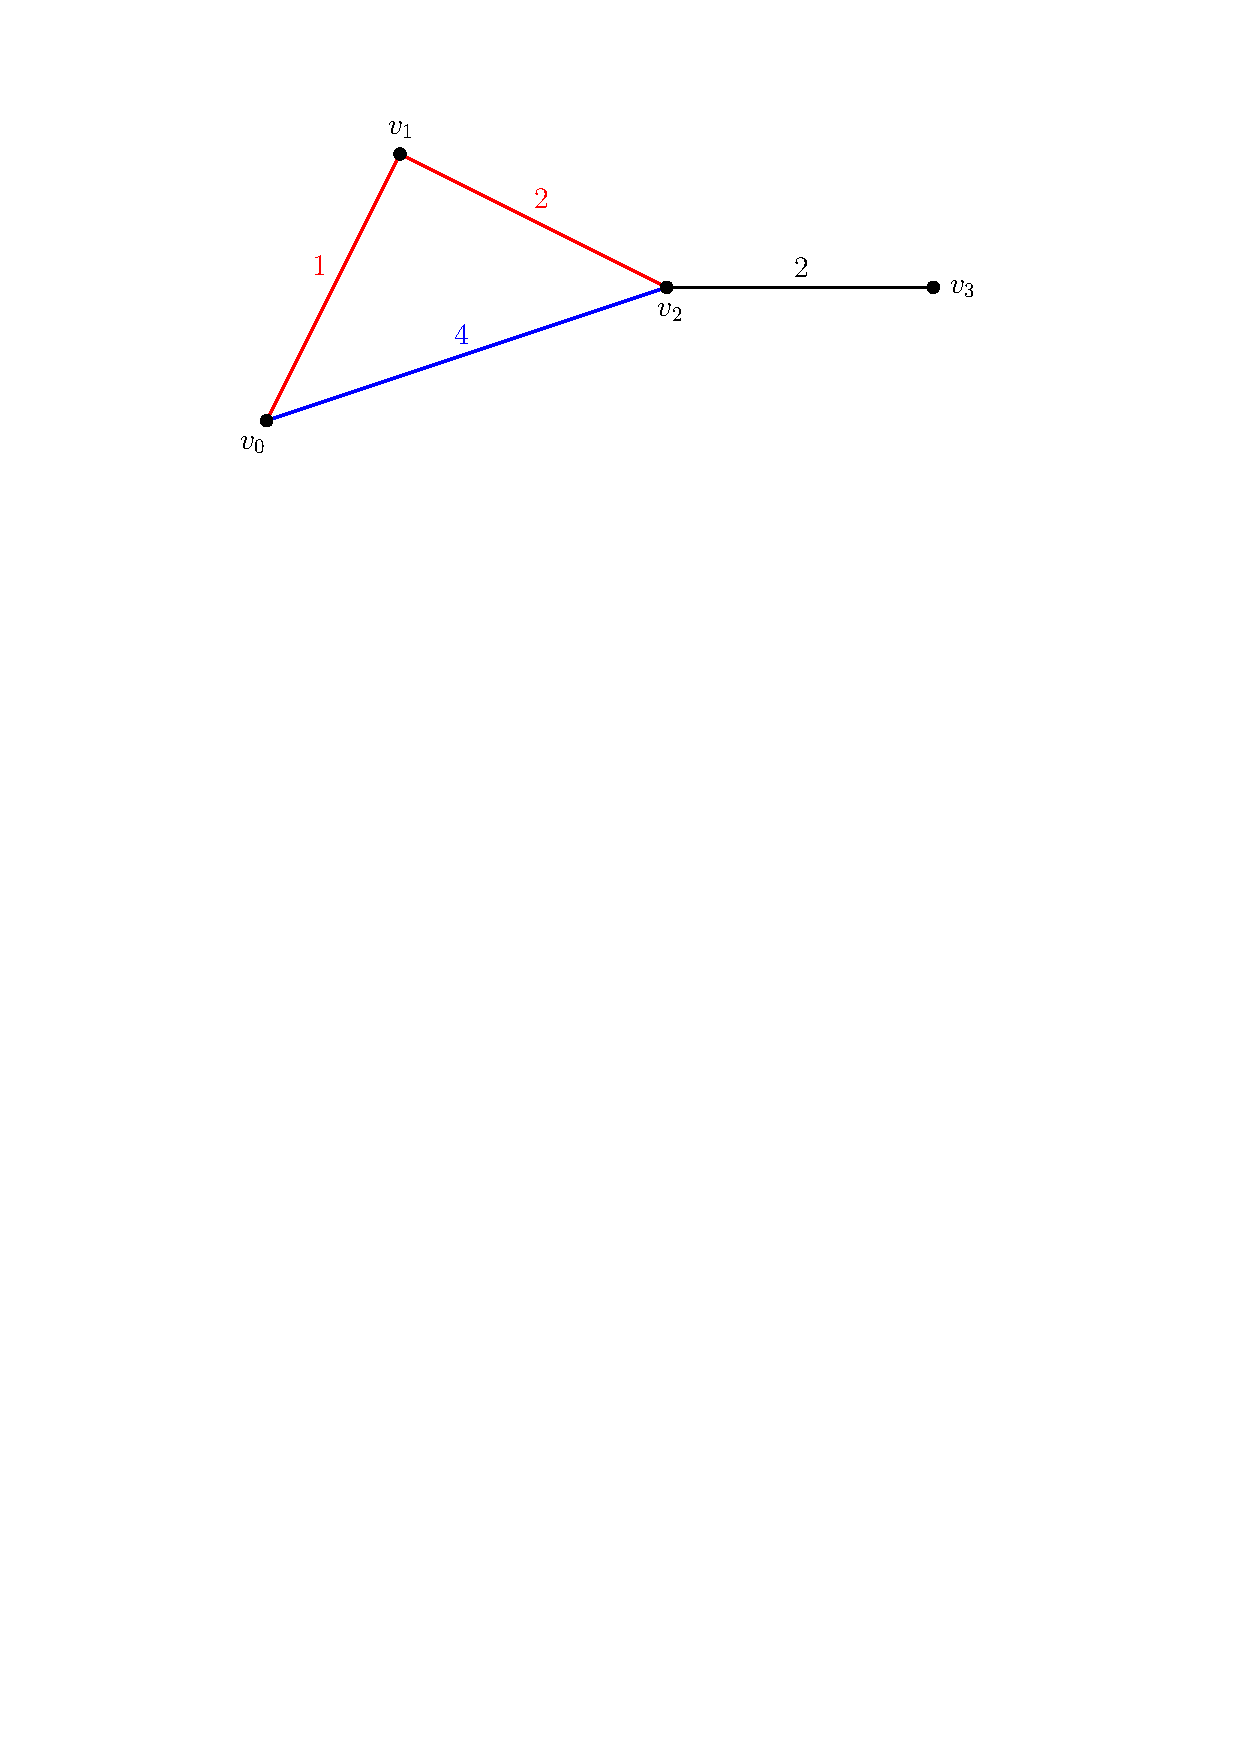
\includegraphics[scale=\graphimgsize]{components/images/ch01_ohod_graf.pdf}
    \caption{Příklad ohodnoceného grafu.}
    \label{fig:ohod_graf}
\end{figure}
Nabízí se varianta převést ohodnocený graf na neohodnocený tak, že rozdělíme hranu na takový počet (neohodnocených) hran, kolik činí její původní váha. V čistě teoretické rovině se jedná o funkční řešení, neboť na nově vzniklý graf již lze aplikovat např. BFS, které jsme popsali v sekci \ref{sec:bfs}. Ne každý graf však musí mít "malé" váhy hran. Pokud bychom vzali např. graf, kde váhy hran jsou v řádech tisíců, bude pro BFS potřeba provést zbytečně mnoho práce, neboť pro zpracování jedné ohodnocené hrany bude třeba provést tisíce iterací.

Jedním z nejznámějších algoritmů v tomto ohledu je tzv. \emph{Dijkstrův algoritmus}, který popsal v roce 1958 holandský informatik \emph{Edsger Wybe Dijkstra}.\footnote{Jedná se o holandské jméno, čteme "dajkstra".} Podobně jako u BFS a DFS, i zde budeme postupně \emph{otevírat} a \emph{uzavírat} vrcholy, přičemž každý uzavřeme \emph{nejvýše jednou}, avšak je třeba mít na paměti důležitou věc.
\importantbox{První nalezená cesta do libovolného vrcholu již nemusí být nutně nejkratší. Cestu do daného vrcholu bude třeba postupně vylepšovat.}
Zaměřme se na grafy, jejichž váhy hran jsou nezáporné. Záporně ohodnocené hrany mohou způsobovat problémy, neboť mezi určitou dvojicí vrcholů by již nemusela nutně existovat nejkratší cesta. Např. v obrázku \ref{fig:zapor_ohod_graf} si lze všimnout, že mezi vrcholy $v_0$ a $v_4$ neexistuje nejratší cesta konečné délky, neboť cyklus $(v_1, v_3, v_2, v_1)$ lze projít libovolněkrát, přičemž každým průchodem se zkrátí o $3$. Odpověď na délku nejrakší cesty mezi těmito vrcholy by tak musela být $-\infty$.
\begin{figure}[h]
    \centering
    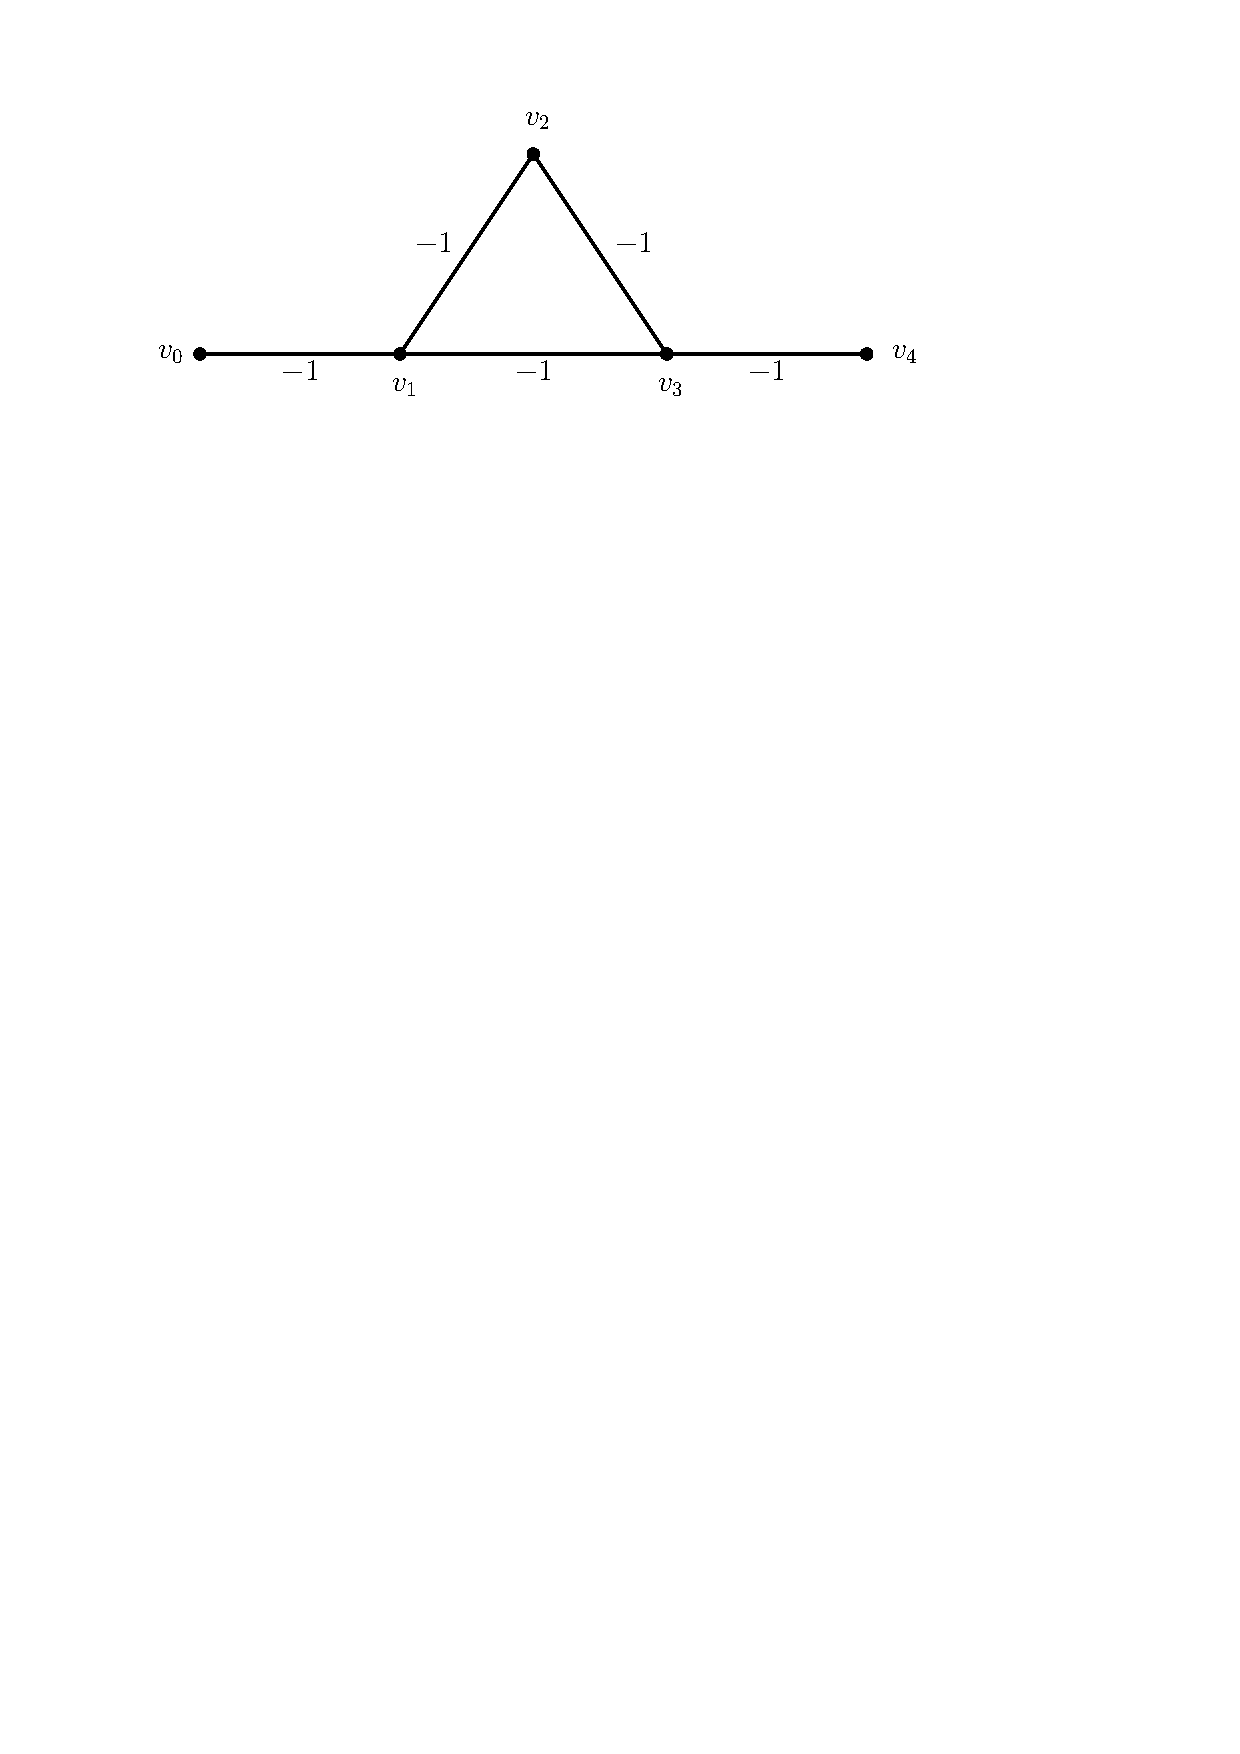
\includegraphics[scale=\graphimgsize]{components/images/ch01_zapor_ohod_graf.pdf}
    \caption{Graf, kde mezi $v_0$ a $v_4$ neexistuje (konečná) nejkratší cesta.}
    \label{fig:zapor_ohod_graf}
\end{figure}
Podobným grafům se tak chceme vyhnout, neboť by naše úvahy pak již nemusely fungovat (cestu mezi vrcholy bychom mohli potenciálně do nekonečně vylepšovat a algoritmus by se tak nikdy nezastavil).

V dalších odstavcích budeme váhu hrany vedoucí z vrcholu $u$ do vrcholu $v$ značit $\ell(u,v)$.
\begin{pseudo}{Dijkstra}[Nezáporně ohodnocený graf $G=(V,E)$ a počáteční vrchol $v_0\in V$.][Seznam vzdáleností $D$.]
    \Comment{Inicializace}
    \begin{For}{všechny vrcholy $v\in V$}
        $stav(v)\gets$ \textit{nenalezený}\\
        $D(v)\gets\infty$\\
    \end{For}
    $stav(v_0)\gets$ \textit{otevřený}\\
    $D(v_0)\gets 0$\\
    \begin{While}{existují otevřené vrcholy}
        \Comment{Kandidát na nejkraší cestu do sousedních vrcholů}
        $v\gets$ otevřený vrchol s nejmenším $D$\\

        \begin{For}{všechny sousedy $w\in V$ vrcholu $v$}
            \Comment{Našli jsme lepší cestu}
            \begin{If}{$D(v)+\ell(v,w)<D(w)$}
                $D(w)\gets D(v)+\ell(v,w)$\\
                $stav(w)\gets$ \textit{otevřený}
            \end{If}
        \end{For}
        $stav(v)\gets$ \textit{uzavřený}
    \end{While}
\end{pseudo}
\begin{figure}[h]
    \centering
    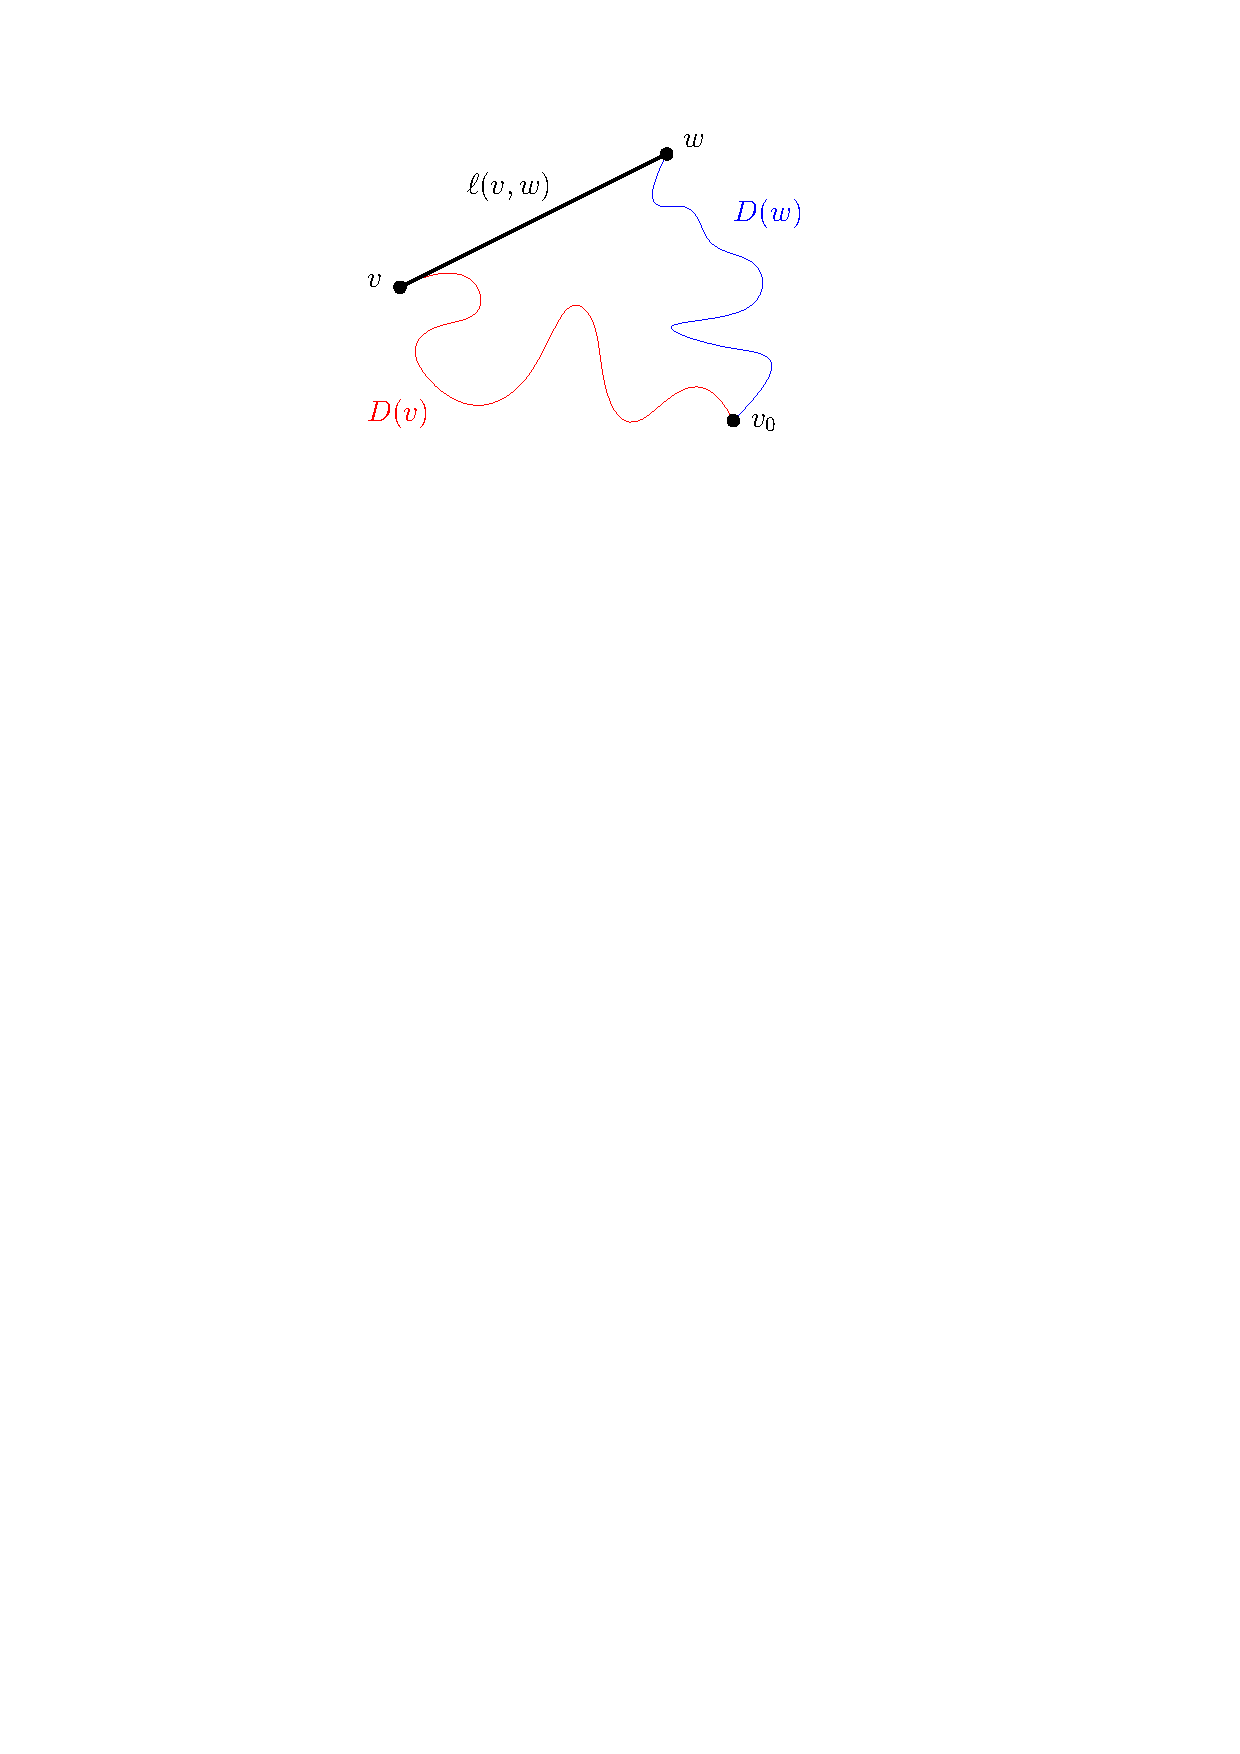
\includegraphics[scale=\graphimgsize]{components/images/ch01_dijkstra_kratsi_cesta.pdf}
    \caption{Znázornění situace v průběhu Dijkstrova algoritmu.}
    \label{fig:dijkstra_kratsi_cesta}
\end{figure}

\subsubsection{Správnost Dijkstrova algoritmu}

Nejprve je dobré si uvědomit, proč algoritmus vlastně funguje. Kdykoliv uzavíráme vrchol (tzn. vybereme vrchol s nejmenší hodnotou $D(v)$), pak se spoléháme na to, že $D(v)$ opravdu odpovídá v daný moment délce nejkraší cesty z $v_0$ do $v$. Ale proč to tak musí být?

Zkusme uvážit opačnou situaci, tzn. kdyby nastalo, že jsme vybrali nějaký vrchol $v$, jehož $D(v)$ neodpovídá délce nejkratší cesty. Pak by musel existovat nějaký sousední vrchol $u$ vrcholu $v$, přes nějž vede nejkratší cesta, jejíž délka je $D(u)+\ell(u,v)$ (viz obrázek \ref{fig:dijkstra_vyber_vrcholu}). To znamená, že $D(v)>D(u)+\ell(u,v)$. Jenže v takovou chvíli by si algoritmus nutně musel vybrat vrchol $u$ místo vrcholu $v$, protože
\[D(v)>D(u)+\ell(u,v)\stackrel{\texttt{*}}{>}D(u).\]
V kroku označeném \texttt{*} vycházíme právě z toho, že váhy hran jsou nezáporné, tj. $\ell(u,v)>0$ (proto tento argument funguje). Tedy stručně řečeno\footnote{Nebo spíš napsáno?}, pokud $D(v)$ neodpovídá délce nejkratší cesty, pak musí existovat jiný vrchol $u$ s nižším $D(u)$.
\begin{figure}[h]
    \centering
    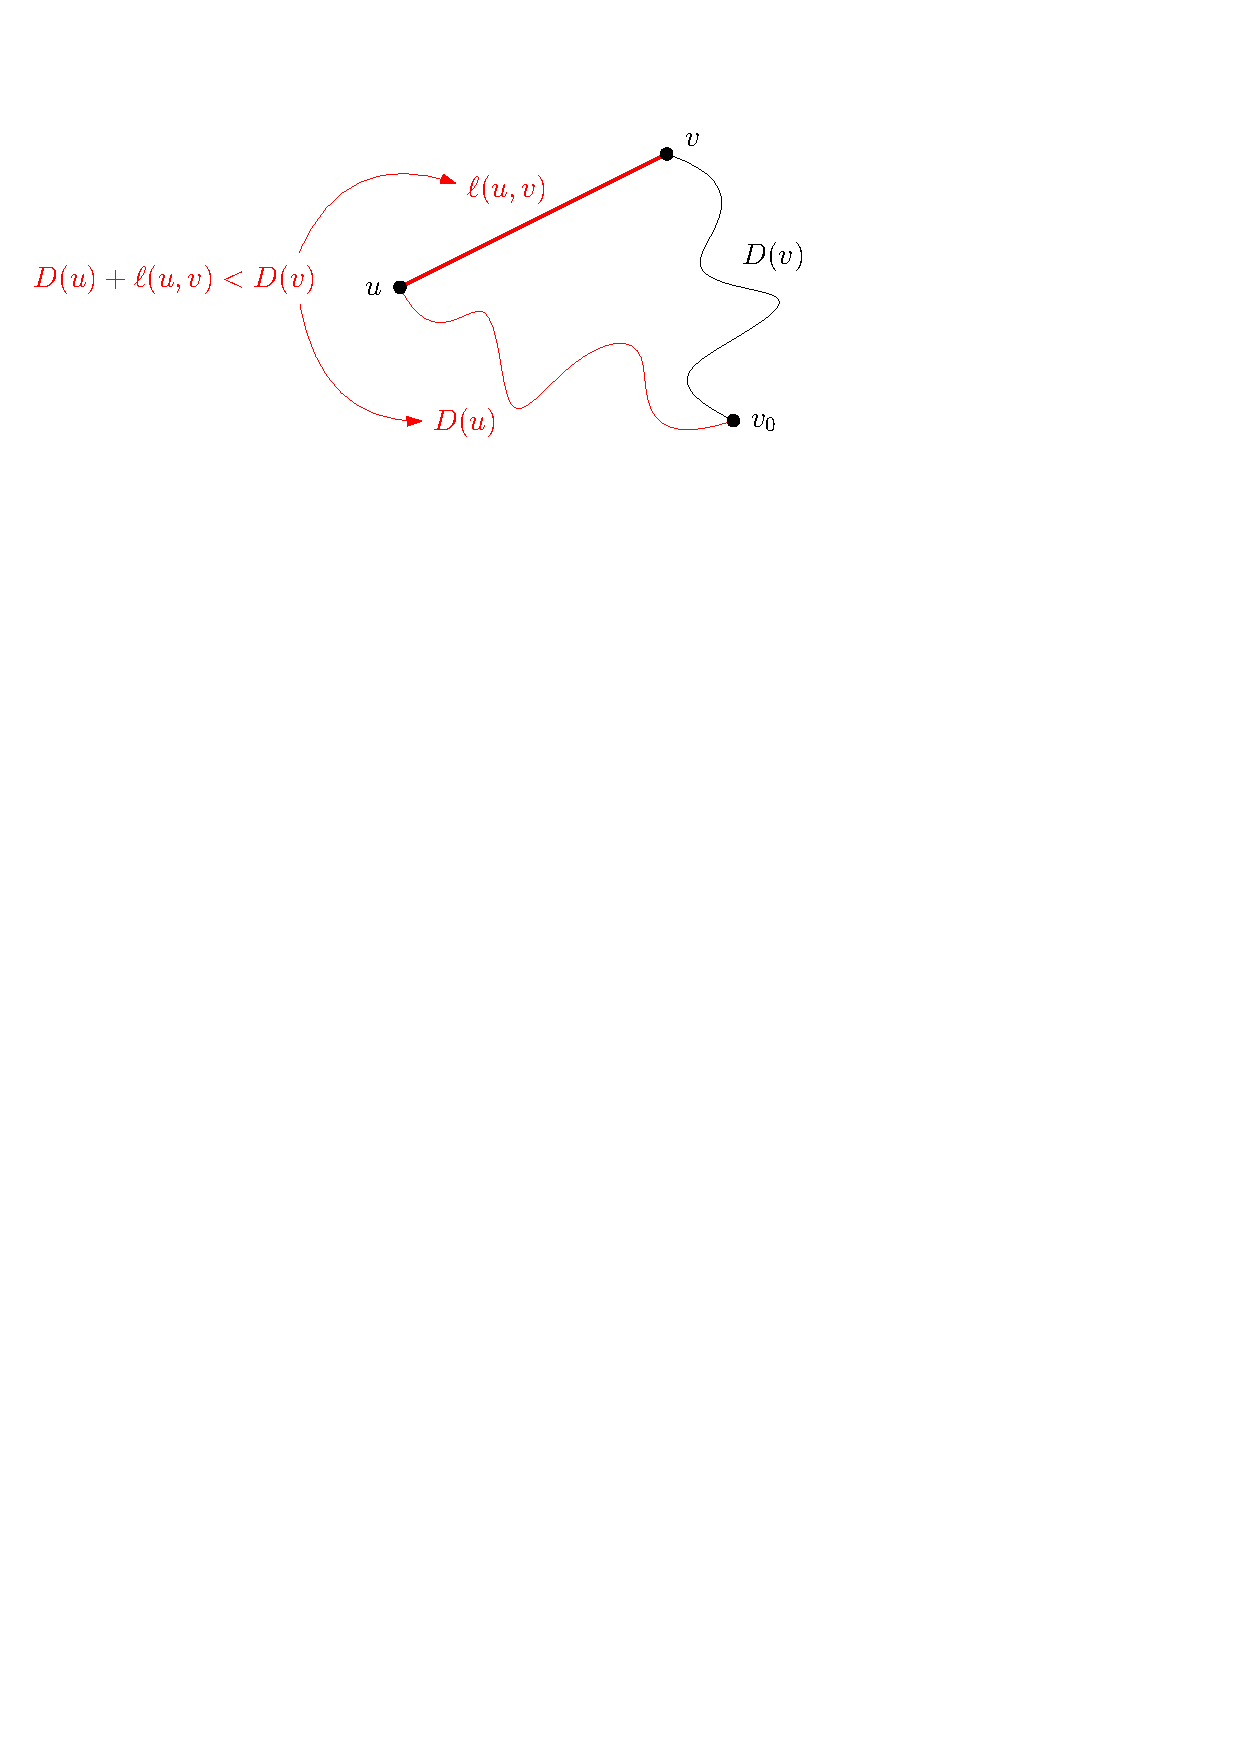
\includegraphics[scale=\graphimgsize]{components/images/ch01_dijkstra_vyber_vrcholu.pdf}
    \caption{Situace při výběru vrcholu $v$, kdy $D(v)$ neodpovídá délce nejkratší cesty.}
    \label{fig:dijkstra_vyber_vrcholu}
\end{figure}

\subsubsection{Časová složitost Dijkstrova algoritmu}

Zbývá nám ještě analyzovat časovou složitost. Pokud se zpětně podíváme na pseudokód algoritmu, lze si všimnout, že podstatnou roli bude hrát vybírání vrcholu s minimální hodnotou $D(v)$. Nabízí se tak otázka, jak danou operaci implementovat. První varintou je hodnoty $D$ realizovat jako prostý \emph{seznam (popř. pole)}.
\begin{theorem}[Dijkstra se seznamem]
    Dijkstrův algoritmus, kde hodnoty $D$ ukládáme do seznamu (pole), doběhne v čase $\bigO{n^2+m}$.
\end{theorem}
\begin{proof}
    \begin{itemize}
        \item Inicializace zabere $\bigO{n}$ (máme $n$ vrcholů).
        \item Každý vrchol uzavřeme opět nejvýše jednou, tzn. vnější cyklus se provede $\bigO{n}$-krát.
        \item Hledání minimálního $D$ zabere v rámci každé iterace čas $\bigO{n}$.
        \item Stejně jako u BFS a DFS, i zde každou hranu zkontroluji nejvýše dvakrát (záleží, zda graf $G$ je orientovaný), tzn. $\bigO{2m}=\bigO{m}$.
    \end{itemize}
    Celkově tedy máme
    \[\overbrace{\bigO{n}}^{\text{Init}}+\underbrace{\bigO{n}\cdot\bigO{n}}_{\text{Výběr minima}}+\bigO{m}=\bigO{n^2+n+m}=\bigO{n^2+m}.\]
\end{proof}
Kvadratická časová složitost není úplně zlá, ale můžeme si ještě trochu přilepšit. Pokud si vzpomeneme na binární haldu z oddílu \ref{sec:halda}, všimneme si v konečném důsledku, že při použití v Dijkstrově algoritmu se některé operace zrychlí.
\begin{theorem}[Dijkstra s haldou]
    Dijkstrův algoritmus, kde hodnoty $D$ ukládáme do binární haldy, doběhne v čase $\bigO{(n+m)\cdot\log{n}}$.
\end{theorem}
\begin{proof}
    Inicializace trvá zase $\bigO{n}$. Při operacích s binární haldou víme, jak dlouho potrvají (vit tabulka \ref{tab:halda_pole_operace}). Akorát si nyní musíme rozmyslet, kdy se která operace provádí.
    \begin{itemize}
        \item Při \emph{otevírání} vrcholu provádíme v haldě operaci \textsc{Insert}\footnote{Náš odhad $\bigO{n\log{n}}$ by šel dokonce zlepšit i na $\bigO{n}$, když do něj započítáme fakt, že hladin v haldě je ze začátku 0 a postupně přibývají (tzn. není jich z počátku "moc"), ale celkový odhad složitosti by vyšel stejně a navíc odvození tohoto faktu je již trochu náročnější.}. Celkově vložíme do haldy max. všech $n$ vrcholů, což potrvá $n\cdot\bigO{\log{n}}=\bigO{n\log{n}}$.
        \item Při \emph{uzavírání} vrcholu provádíme operaci \textsc{ExtractMin} (opět max. $n$-krát), tj. $n\cdot\bigO{\log{n}}=\bigO{n\log{n}}$.
        \item Při \emph{aktualizaci vzdálenosti} $D(v)$ provádíme \textsc{Decrease} (tato hodnota se nikdy nemůže zvýšit). To provádíme vždy při kontrole sousedů (tzn. daných hran), kterých je pro všechny vrcholy dohromady max. $\bigO{m}$ (stejný argument jako při započítávání hran). Tzn. $m\cdot\bigO{\log{n}}=\bigO{m\log{n}}$.
    \end{itemize}
    Po sečtení dostaneme
    \begin{align*}
        \bigO{n+n\log{n}+n\log{n}+m\log{n}}&=\bigO{n+2n\log{n}+m\log{n}}\\
        &=\bigO{n+n\log{n}+m\log{n}}\\
        &=\bigO{n\log{n}+m\log{n}}\\
        &=\bigO{(n+m)\cdot\log{n}}.
    \end{align*}
\end{proof}
Ačkoliv to není úplně zjevné, výraz $(n+m)\cdot\log{n}$ roste o dost pomaleji oproti $n^2+m$, tedy binární haldou si skutečně pomůžeme oproti seznamu.

Závěrem zde je ještě uveďme, že často nehledáme cestu do všech vrcholů, ale pouze mezi nějakou konkrétní dvojicí. V takovou chvíli můžeme výpočet algoritmu zarazit ve chvíli, kdy narazíme na cílový vrchol, protože jak již víme, při otevírání vrcholu je $D(v)$ skutečná délka nejkratší cesty. V tomto případě je možné ještě dále urychlit hledání nejkratší cesty, neboť Dijkstrův algoritmus může pak provádět hodně nadbytečné práce. Na to se podíváme v další sekci \ref{sec:astar}.